%% ----------------------------------------------------------------------------
%%  §9.1  Il teorema fondamentale del calcolo integrale
%% ----------------------------------------------------------------------------
\section{Il teorema fondamentale del calcolo integrale}
\label{sec:teorema-fondamentale}

Ci proponiamo di mettere in evidenza una relazione tra integrali e derivate che avrà
applicazioni in tutto il calcolo integrale. L'idea è di far variare uno degli estremi
di integrazione e di studiare l'integrale come \emph{funzione} di tale estremo.

\subsection{La funzione integrale}

Sia $f$ una funzione integrabile nell'intervallo $[a,b]$. Per il
\cref{lem:sottointervallo}, $f$ è integrabile in ogni intervallo $[a,x]$ con
$x\in[a,b]$, e possiamo considerare
\begin{equation}\label{eq:funzione-integrale}
  F(x)=\int_{a}^{x}f(t)\,dt, \qquad x\in[a,b] ,
\end{equation}
con $F(a)=0$ per la convenzione \eqref{eq:estremi-invertiti}. Abbiamo indicato la
variabile di integrazione con $t$ invece che con $x$: è un puro scambio di simboli,
perché la variabile di integrazione è muta, ma ci permette di riservare la lettera $x$
al secondo estremo. Per ogni $x$ l'integrale è un numero, e al variare di $x$ si ottiene
una funzione, detta \emph{funzione integrale} di $f$ con punto iniziale
$a$.\index{funzione!integrale} Ad esempio, per le \eqref{eq:integrale-x} e
\eqref{eq:integrale-x2},
\begin{equation}\label{eq:funzioni-integrali-esempi}
  \int_{0}^{x}t\,dt=\frac{x^{2}}2, \qquad \int_{0}^{x}t^{2}\,dt=\frac{x^{3}}3
  \qquad (x\ge0) .
\end{equation}
In entrambi i casi la derivata della funzione integrale ($x$ e $x^{2}$) è la funzione
integranda calcolata nel secondo estremo. È il fenomeno osservato
nell'\cref{oss:indizio-tfc}; vedremo che vale in generale.

Se si sceglie un altro punto iniziale $c\in[a,b]$, per l'additività
(\cref{teo:additivita}) si ha $\int_{c}^{x}f=\int_{a}^{x}f-\int_{a}^{c}f=F(x)-F(c)$: le
funzioni integrali con punti iniziali diversi differiscono per una costante.

\begin{proposizione}[La funzione integrale è lipschitziana]\label{prop:integrale-lipschitz}
Sia $f$ integrabile in $[a,b]$, con $\abs{f(t)}\le K$ per ogni $t\in[a,b]$. Allora
\begin{equation}\label{eq:integrale-lipschitz}
  \abs{F(x)-F(x')}\le K\,\abs{x-x'} \qquad\perogni x,x'\in[a,b] ;
\end{equation}
in particolare $F$ è uniformemente continua in $[a,b]$.
\end{proposizione}

\begin{schema}
\Ipotesi{$f$ integrabile in $[a,b]$; \ $\abs f\le K$.}
\Tesi{$F$ lipschitziana con costante $K$, e quindi uniformemente continua.}
\end{schema}

\begin{strategia}
Per l'additività, $F(x)-F(x')$ è l'integrale di $f$ tra $x'$ e $x$; lo si stima con il
valore assoluto e il confronto con la costante $K$.
\end{strategia}

\begin{dimostrazione}
Siano $x'<x$ (se $x=x'$ non c'è nulla da dimostrare, e il caso $x<x'$ è simmetrico).
Per l'additività, $F(x)-F(x')=\int_{x'}^{x}f(t)\,dt$, e per il \cref{teo:valore-assoluto}
e il \cref{teo:confronto-integrali},
\[
  \abs{F(x)-F(x')}\le\int_{x'}^{x}\abs{f(t)}\,dt\le\int_{x'}^{x}K\,dt=K\,(x-x') .
\]
L'uniforme continuità segue dalla \cref{prop:lipschitz-uniforme}.
\end{dimostrazione}

La funzione integrale è dunque sempre continua, anche quando $f$ non lo è; ma può non
essere derivabile. Ad esempio, se in $[-1,1]$ si pone $f(t)=-1$ per $t<0$ e $f(t)=1$ per
$t\ge0$, si trova $\int_{-1}^{x}f(t)\,dt=-(x+1)$ per $x\le0$ e $-1+x$ per $x\ge0$ (il
valore di $f$ nel solo punto $0$ non conta, per l'\cref{es:valore-in-un-punto}),
cioè $F(x)=\abs x-1$, che non è derivabile in $0$: il salto della funzione integranda
diventa un punto angoloso della funzione integrale. Il teorema seguente afferma che,
dove $f$ è continua, $F$ è derivabile.

\subsection{Il teorema fondamentale}

\begin{teorema}[fondamentale del calcolo integrale]\label{teo:fondamentale}
\index{teorema!fondamentale del calcolo integrale}
Sia $f$ una funzione continua nell'intervallo $[a,b]$. La funzione integrale
\eqref{eq:funzione-integrale} è derivabile in $[a,b]$ e la sua derivata vale
\begin{equation}\label{eq:teorema-fondamentale}
  F'(x)=f(x) \qquad\perogni x\in[a,b]
\end{equation}
(negli estremi $a$ e $b$ si intendono la derivata destra e la derivata sinistra).
\end{teorema}

\begin{schema}
\Ipotesi{$f$ continua in $[a,b]$; \ $F(x)=\int_{a}^{x}f(t)\,dt$.}
\Tesi{$F$ derivabile in $[a,b]$ e $F'(x)=f(x)$ per ogni $x$.}
\end{schema}

\begin{strategia}
Dobbiamo calcolare il limite del rapporto incrementale di $F$. Per l'additività,
l'incremento $F(x+h)-F(x)$ è l'integrale di $f$ tra $x$ e $x+h$, e il rapporto
incrementale è quindi la \emph{media integrale} di $f$ sull'intervallo di estremi $x$ e
$x+h$. Il teorema della media la trasforma in un valore $f(\xi_{h})$, con $\xi_{h}$ compreso
tra $x$ e $x+h$; quando $h\to0$ il punto $\xi_{h}$ è costretto a tendere a $x$, e la
continuità di $f$ in $x$ fa il resto. Geometricamente: la striscia di base $h$ aggiunta
al rettangoloide ha un'area molto vicina a quella del rettangolo di altezza $f(x)$.
\end{strategia}

\begin{dimostrazione}
Sia $x\in[a,b]$ e sia $h\neq0$ tale che $x+h\in[a,b]$. Per l'additività
(\cref{teo:additivita}),
\begin{equation}\label{eq:rapporto-funzione-integrale}
  \frac{F(x+h)-F(x)}h=\frac1h\Bigl[\int_{a}^{x+h}f(t)\,dt-\int_{a}^{x}f(t)\,dt\Bigr]
  =\frac1h\int_{x}^{x+h}f(t)\,dt .
\end{equation}
Se $h>0$, l'ultimo membro è la media integrale di $f$ in $[x,x+h]$; se $h<0$, per la
\eqref{eq:estremi-invertiti} esso vale $\frac1{\abs h}\int_{x+h}^{x}f(t)\,dt$, cioè la media
integrale di $f$ in $[x+h,x]$. In entrambi i casi, per il teorema della media
(\cref{teo:media}) applicato alla funzione continua $f$, esiste un punto $\xi_{h}$
dell'intervallo di estremi $x$ e $x+h$ tale che
\begin{equation}\label{eq:rapporto-media}
  \frac{F(x+h)-F(x)}h=f(\xi_{h}), \qquad \abs{\xi_{h}-x}\le\abs h .
\end{equation}
Sia ora $\epsilon>0$. Per la continuità di $f$ in $x$ esiste $\delta>0$ tale che
$\abs{f(t)-f(x)}<\epsilon$ per ogni $t\in[a,b]$ con $\abs{t-x}<\delta$. Se $0<\abs h<\delta$,
allora $\abs{\xi_{h}-x}\le\abs h<\delta$, e quindi
\[
  \Bigl|\frac{F(x+h)-F(x)}h-f(x)\Bigr|=\abs{f(\xi_{h})-f(x)}<\epsilon .
\]
Questo prova che il rapporto incrementale tende a $f(x)$ per $h\to0$ (soltanto da destra
se $x=a$, soltanto da sinistra se $x=b$), cioè la \eqref{eq:teorema-fondamentale}.
\end{dimostrazione}

\begin{figure}[htb]
\centering
\begin{tikzpicture}
\begin{axis}[name=t1, width=0.5\textwidth, height=4.6cm, axis lines=left, xmin=0,
  xmax=4.4, ymin=0, ymax=2.5, xtick={0.5,2.6}, xticklabels={$a$,$x$}, ytick=\empty,
  title={\scriptsize $F(x)$ = area da $a$ a $x$}, clip=false]
  \addplot[draw=none, fill=blu!22, domain=0.5:2.6, samples=50]
    {1.1+0.6*sin(deg(1.3*x))+0.1*x} \closedcycle;
  \addplot[curva, domain=0.3:4.2, samples=100] {1.1+0.6*sin(deg(1.3*x))+0.1*x};
  \node[font=\scriptsize, blu] at (axis cs:1.55,0.6) {$F(x)$};
  \node[font=\scriptsize] at (axis cs:3.7,1.45) {$y=f(t)$};
\end{axis}
\begin{axis}[at={(t1.east)}, anchor=west, xshift=0.7cm, width=0.5\textwidth,
  height=4.6cm, axis lines=left, xmin=0, xmax=4.4, ymin=0, ymax=2.5,
  xtick={2.6,3.2}, xticklabels={$x$,$x+h$}, ytick={1.2183},
  yticklabels={$f(x)$}, title={\scriptsize l'incremento $F(x+h)-F(x)$},
  tick label style={font=\scriptsize}]
  \addplot[draw=none, fill=rame!35, domain=2.6:3.2, samples=30]
    {1.1+0.6*sin(deg(1.3*x))+0.1*x} \closedcycle;
  \draw[blu, thick] (axis cs:2.6,0) rectangle (axis cs:3.2,1.2183);
  \addplot[curva, domain=0.3:4.2, samples=100] {1.1+0.6*sin(deg(1.3*x))+0.1*x};
  \addplot[tratteggio] coordinates {(0,1.2183) (2.6,1.2183)};
\end{axis}
\end{tikzpicture}
\caption{A sinistra, la funzione integrale $F(x)$ come area del rettangoloide da $a$ a
$x$. A destra, l'incremento $F(x+h)-F(x)$ è l'area della striscia in color rame, che
differisce poco da quella del rettangolo $f(x)\,h$ (contorno blu): dividendo per $h$ e
facendo tendere $h$ a zero si ottiene $F'(x)=f(x)$.}
\label{fig:teorema-fondamentale}
\end{figure}

La dimostrazione usa la continuità di $f$ soltanto nel punto $x$ (oltre che per poter
applicare il teorema della media). In effetti vale un risultato più generale, che spiega
il punto angoloso dell'esempio precedente.

\begin{osservazione}[Basta la continuità nel punto]\label{oss:fondamentale-puntuale}
Sia $f$ integrabile in $[a,b]$ e continua in un punto $x_{0}$. Allora $F$ è derivabile
in $x_{0}$ e $F'(x_{0})=f(x_{0})$. Infatti, poiché $\frac1h\int_{x_{0}}^{x_{0}+h}f(x_{0})\,dt
=f(x_{0})$, dalla \eqref{eq:rapporto-funzione-integrale} si ha
\[
  \frac{F(x_{0}+h)-F(x_{0})}h-f(x_{0})=\frac1h\int_{x_{0}}^{x_{0}+h}\bigl[f(t)-f(x_{0})\bigr]dt ,
\]
e se $\abs{f(t)-f(x_{0})}<\epsilon$ per $\abs{t-x_{0}}<\delta$, per $0<\abs h<\delta$ il secondo
membro non supera in valore assoluto $\frac1{\abs h}\,\epsilon\abs h=\epsilon$ (per il
\cref{teo:valore-assoluto} e il confronto). Dove $f$ ha un salto, invece, i rapporti
incrementali destro e sinistro di $F$ tendono ai due limiti laterali di $f$ (con lo
stesso argomento, usando i limiti laterali al posto di $f(x_{0})$), e $F$ ha un punto
angoloso.
\end{osservazione}

Il teorema fondamentale si combina con la regola di derivazione delle funzioni composte.

\begin{corollario}[Estremi variabili]\label{cor:estremi-variabili}
Sia $f$ continua in un intervallo $I$, siano $c\in I$ e $\varphi$ una funzione
derivabile in un intervallo $J$, con valori in $I$. Allora, rispettivamente per ogni
$x\in I$ e per ogni $x\in J$,
\begin{equation}\label{eq:estremi-variabili}
  \frac{d}{dx}\int_{x}^{c}f(t)\,dt=-f(x), \qquad
  \frac{d}{dx}\int_{c}^{\varphi(x)}f(t)\,dt=f\bigl(\varphi(x)\bigr)\,\varphi'(x) .
\end{equation}
\end{corollario}

\begin{schema}
\Ipotesi{$f$ continua nell'intervallo $I$; \ $c\in I$; \ $\varphi:J\to I$ derivabile
($J$ intervallo).}
\Tesi{le due formule \eqref{eq:estremi-variabili}.}
\end{schema}

\begin{strategia}
Con $F(x)=\int_{c}^{x}f$ si ha $\int_{x}^{c}f=-F(x)$ e $\int_{c}^{\varphi(x)}f=F(\varphi(x))$;
basta derivare con il teorema fondamentale e la regola della catena.
\end{strategia}

\begin{dimostrazione}
Sia $F(x)=\int_{c}^{x}f(t)\,dt$. Per la \eqref{eq:estremi-invertiti},
$\int_{x}^{c}f=-F(x)$, la cui derivata è $-f(x)$ per il \cref{teo:fondamentale} (applicato
in un intervallo chiuso e limitato contenuto in $I$ che contenga $c$ e $x$, con $x$ al suo
interno se $x$ non è un estremo di $I$). Inoltre
$\int_{c}^{\varphi(x)}f=F(\varphi(x))$, e per il \cref{teo:derivata-composta} la sua derivata
è $F'(\varphi(x))\,\varphi'(x)=f(\varphi(x))\,\varphi'(x)$.
\end{dimostrazione}

Ad esempio, $\frac{d}{dx}\int_{0}^{x^{2}}e^{-t^{2}}dt=2x\,e^{-x^{4}}$: la derivata si calcola
senza conoscere alcuna formula esplicita per l'integrale. È proprio questo il punto di
forza del teorema: la funzione $\int_{0}^{x}e^{-t^{2}}dt$, che non si esprime mediante
funzioni elementari, ha comunque derivata nota, ed è quindi crescente, con un flesso
nell'origine, dove $e^{-x^{2}}$ ha il massimo (\cref{fig:funzione-integrale}). Il programma
seguente calcola numericamente la funzione integrale e ne verifica la derivata con il
rapporto incrementale simmetrico; come riferimento usa la funzione \texttt{erf} di Python,
definita proprio come $\frac2{\sqrt\pi}\int_{0}^{x}e^{-t^{2}}dt$.

\begin{python}[La funzione integrale di $e^{-t^2}$ e la sua derivata]
import math

f = lambda t: math.exp(-t * t)

def F(x, n=2000):
    """Funzione integrale int_0^x f(t) dt (punto medio)."""
    h = x / n
    return h * sum(f((k + 0.5) * h) for k in range(n))

h = 1e-3
print("  x      F(x)  sqrt(pi)/2 erf(x)   rapp. incr.     f(x)")
for x in (0.0, 0.5, 1.0, 1.5, 2.0):
    rif = math.sqrt(math.pi) / 2 * math.erf(x)
    d = (F(x + h) - F(x - h)) / (2 * h)
    print(f"{x:4.1f}  {F(x):.6f}      {rif:.6f}      {d:.6f}"
          f"   {f(x):.6f}")
\end{python}
\begin{risultato}
  x      F(x)  sqrt(pi)/2 erf(x)   rapp. incr.     f(x)
 0.0  0.000000      0.000000      1.000000   1.000000
 0.5  0.461281      0.461281      0.778801   0.778801
 1.0  0.746824      0.746824      0.367880   0.367879
 1.5  0.856188      0.856188      0.105399   0.105399
 2.0  0.882081      0.882081      0.018316   0.018316
\end{risultato}

\begin{figure}[htb]
\centering
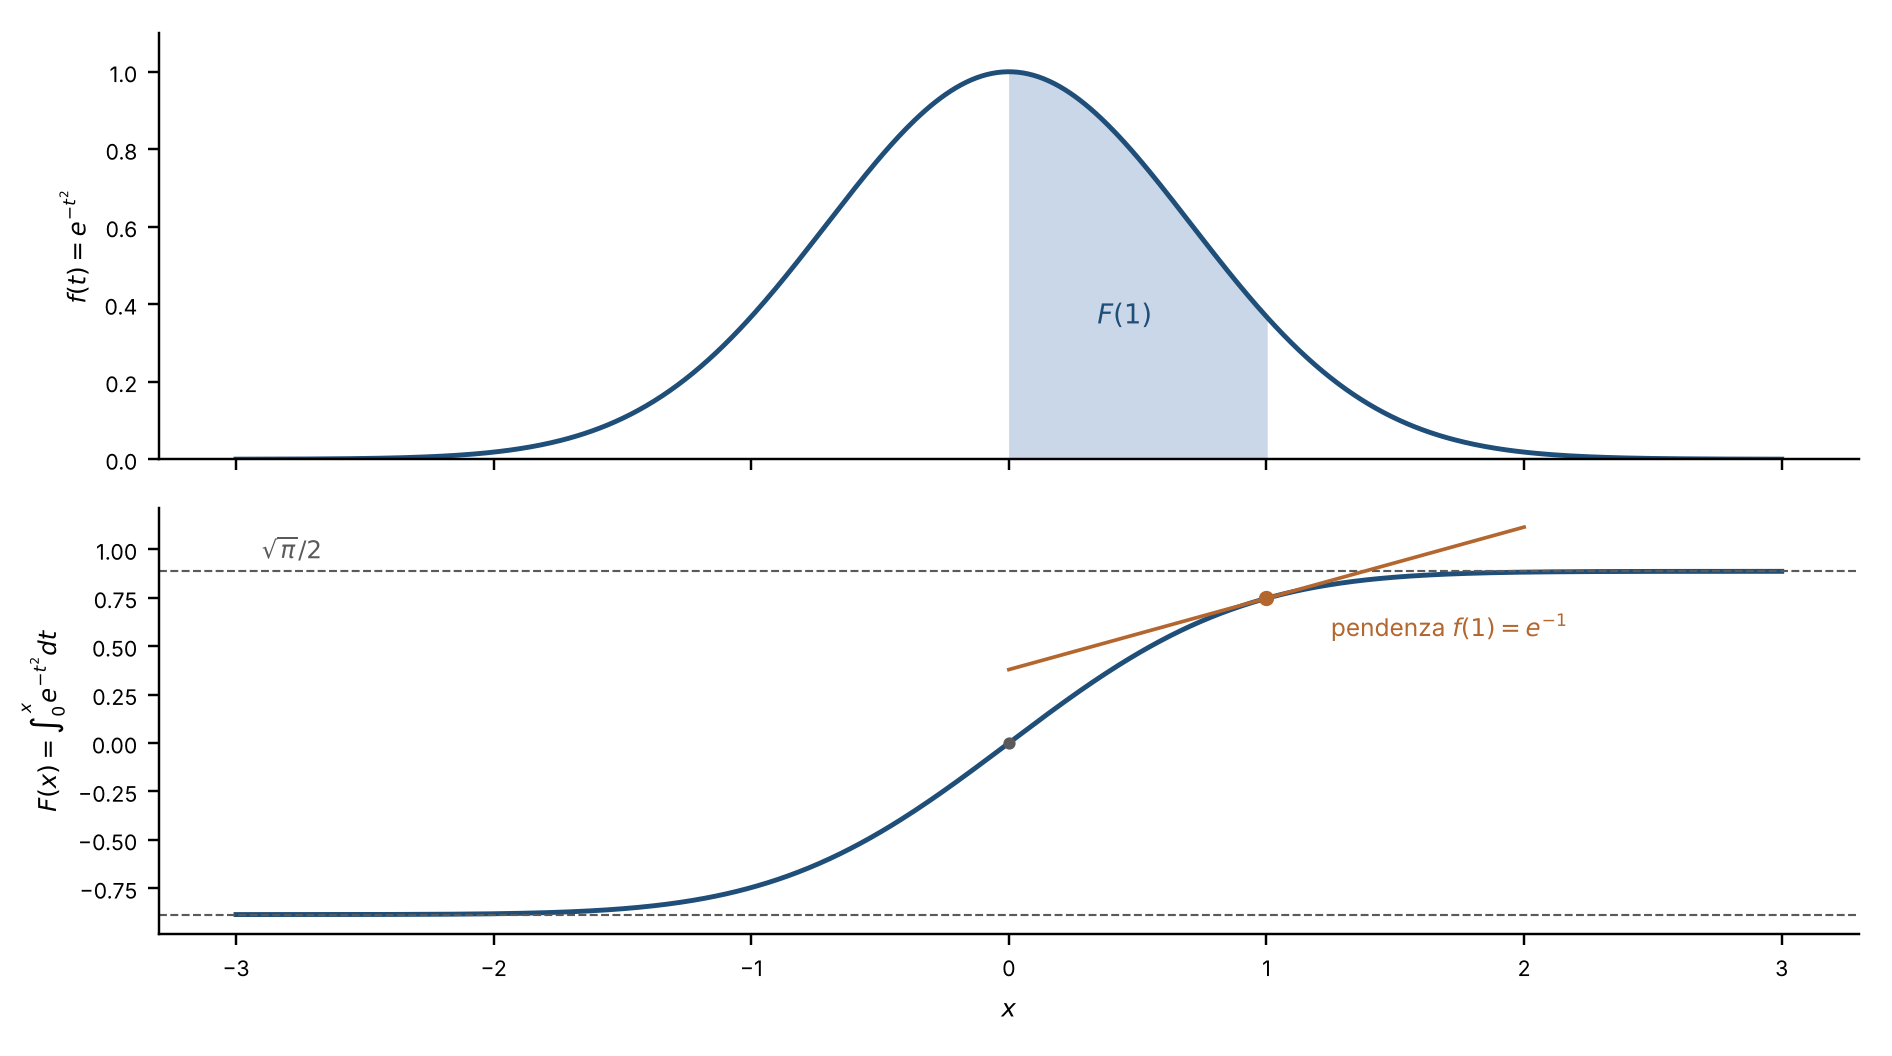
\includegraphics[width=\textwidth]{figure/funzione_integrale.png}
\caption{In alto, la funzione $f(t)=e^{-t^{2}}$ con l'area da $0$ a $x=1$; in basso, la
sua funzione integrale $F(x)=\int_{0}^{x}e^{-t^{2}}dt$, con la retta tangente in $x=1$, di
pendenza $f(1)=e^{-1}$. Dove $f$ è massima, $F$ ha il flesso; l'esistenza degli asintoti
orizzontali sarà dimostrata nel \cref{sec:impropri}, mentre il loro valore $\pm\frac{\sqrt\pi}2$ si
calcola in un corso di Analisi Matematica~2
(\texttt{python/fig\_funzione\_integrale.py}).}
\label{fig:funzione-integrale}
\end{figure}

\begin{notastorica}[Newton, Leibniz e la disputa sulla priorità]
Il legame tra il problema delle tangenti e quello delle aree fu intravisto da diversi
matematici del Seicento: Evangelista Torricelli, James Gregory e soprattutto Isaac
Barrow, che nelle \emph{Lectiones geometricae} (1670) ne diede una formulazione
geometrica. Furono però Isaac Newton, intorno al 1665--1666, e Gottfried Wilhelm
Leibniz, a Parigi, intorno al 1675, a farne lo strumento di un calcolo generale, con
notazioni e regole valide per tutte le curve (Newton, nel 1669, succedette proprio a
Barrow sulla cattedra lucasiana di Cambridge). Nello stesso 1669 Newton raccolse i suoi
metodi nel \emph{De analysi}, stampato soltanto nel 1711: vi mostrava che l'area sotto
una curva, pensata come funzione dell'ascissa, cresce con velocità uguale all'ordinata
(il nostro $F'=f$), e calcolava le aree sviluppando in serie e integrando termine a
termine. Newton
comunicò il risultato a Leibniz in forma cifrata, con l'anagramma dell'epigrafe, nella
lettera del 24 ottobre 1676; Leibniz pubblicò per primo, nel 1684 e nel 1686, sugli
\emph{Acta Eruditorum}. Ne seguì una violenta disputa sulla priorità, che la Royal
Society, presieduta da Newton, chiuse nel 1712 a favore del suo presidente (il rapporto
fu pubblicato nel 1713 nel \emph{Commercium epistolicum}) e che divise
per un secolo i matematici inglesi da quelli del continente. Oggi si riconosce che le
due scoperte furono indipendenti. La parola «integrale» comparve a stampa nel 1690, in
una memoria di Jakob Bernoulli sugli \emph{Acta Eruditorum}; Leibniz, che parlava di
\emph{calculus summatorius}, adottò poi il nome \emph{calculus integralis} proposto da
Johann Bernoulli. La dimostrazione rigorosa che abbiamo seguito, basata sul teorema
della media, è dovuta a Cauchy (1823). Avendo definito l'integrale come limite di somme
(si veda la nota storica del \S\ref{sec:integrale-definito}), Cauchy dovette
\emph{dimostrare} ciò che per i predecessori, per i quali integrare significava trovare
una primitiva, era quasi una definizione.
\end{notastorica}
